% ===========================================================================
% Part II - Density-Based Learning (Experiments 5-6)
% ===========================================================================

\part{Density-Based Learning}

% ---------------------------------------------------------------------------
\chapter{DBSCAN}\label{exp:05}

\runninghead{Experiment 5: DBSCAN}

\quickfacts
  {Dataset}{USGS earthquakes 2023 (\texttt{data/earthquakes.csv}); 7,638 events with magnitude $\ge$ 4.5}
  {Key parameters}{$\varepsilon$ = 0.03 rad ($\approx$ 191 km), \texttt{min\_samples} = 10, haversine metric on radian coordinates}
  {Headline result}{55 clusters, 13.5\% noise; largest clusters match the Philippines, Papua New Guinea, Tonga, Japan and Turkey}

\section{Objective}
Detect dense groups and noise using DBSCAN without specifying the number of clusters in
advance, applied to real spatial data.

\section{Suggested Dataset}
Real USGS earthquake catalogue 2023 (\texttt{data/earthquakes.csv}): 16,190 global events at
magnitude $\ge$ 4.0, filtered to the 7,638 events at magnitude $\ge$ 4.5. Coordinates are
converted to radians and clustered with the haversine (great-circle) metric.

\section{Required Libraries}
scikit-learn, numpy, pandas, matplotlib.

\section{Brief Theory}
DBSCAN defines clusters as connected regions of density. For a point $p$:
\begin{itemize}
  \item \textbf{$\varepsilon$-neighborhood:} $N_\varepsilon(p) = \{q : \mathrm{dist}(p,q) \le \varepsilon\}$;
  \item \textbf{core point:} $|N_\varepsilon(p)| \ge \texttt{min\_samples}$;
  \item \textbf{border point:} inside the $\varepsilon$-neighborhood of a core point but not core itself;
  \item \textbf{noise:} neither core nor border (label $-1$).
\end{itemize}
Clusters grow by chaining density-reachable core points, so arbitrary shapes can be
discovered and no $K$ is required. A single global $\varepsilon$ struggles when densities
vary. Because latitude/longitude are spherical coordinates, the \textbf{haversine}
(great-circle) metric is used with radian inputs; $\varepsilon$ is then expressed in radians
($0.03$ rad $\times$ 6371 km $\approx$ 191 km).

\section{Procedure}
\begin{enumerate}
  \item Load the catalogue and filter to magnitude $\ge 4.5$ (well-recorded events).
  \item Convert latitude/longitude to radians for the haversine metric.
  \item Choose $\varepsilon$ from the $k$-distance graph ($k = 10$); the knee is at 0.03 rad.
  \item Fit DBSCAN and count clusters and noise events.
  \item Show a parameter-sensitivity table for at least two settings.
  \item Visualize the epicenters and validate the largest clusters against known seismic regions.
\end{enumerate}

\section{Reference Implementation}
\begin{codebox}[title={$\varepsilon$ from the $k$-distance knee, then DBSCAN with the haversine metric}]
X_rad = np.radians(quakes[['latitude', 'longitude']].values)
nbrs = NearestNeighbors(n_neighbors=10, metric='haversine').fit(X_rad)
k_distances = np.sort(nbrs.kneighbors(X_rad)[0][:, -1])   # knee ~0.03 rad

dbscan = DBSCAN(eps=0.03, min_samples=10, metric='haversine')
db_labels = dbscan.fit_predict(X_rad)
\end{codebox}

\section{Evaluation / Expected Output}
\begin{table}[htbp]
  \centering
  \caption{DBSCAN parameter sensitivity (\texttt{min\_samples} = 10).}
  \begin{tabular}{|l|r|r|r|}
    \hline
\rowcolor{mlblue!8}    \textbf{$\varepsilon$ (rad)} & \textbf{approx.\ km} & \textbf{clusters} & \textbf{noise} \\
    \hline
    0.02 & 127 & 70 & 21.2\% \\
\hline
    \best{0.03 (selected)} & \best{191} & \best{55} & \best{13.5\%} \\
\hline
    0.05 & 319 & 50 & 5.7\% \\
    \hline
  \end{tabular}
\end{table}

\begin{table}[htbp]
  \centering
  \caption{Largest DBSCAN clusters and their dominant region (real-world validation).}
  \begin{tabular}{|l|r|r|l|}
    \hline
\rowcolor{mlblue!8}    \textbf{Cluster} & \textbf{Events} & \textbf{Center lat/lon} & \textbf{Dominant region} \\
    \hline
    4 & 1,629 & 6.1, 126.1 & Philippines \\
\hline
    0 & 1,068 & $-12.5$, 160.0 & Papua New Guinea \\
\hline
    1 & 947 & $-24.0$, $-154.5$ & Tonga \\
\hline
    5 & 895 & 30.8, 145.0 & Japan region \\
\hline
    2 & 253 & $-57.8$, $-26.3$ & South Sandwich Islands \\
\hline
    8 & 207 & 37.7, 37.2 & Turkey \\
    \hline
  \end{tabular}
\end{table}

\begin{figure}[htbp]
  \centering
  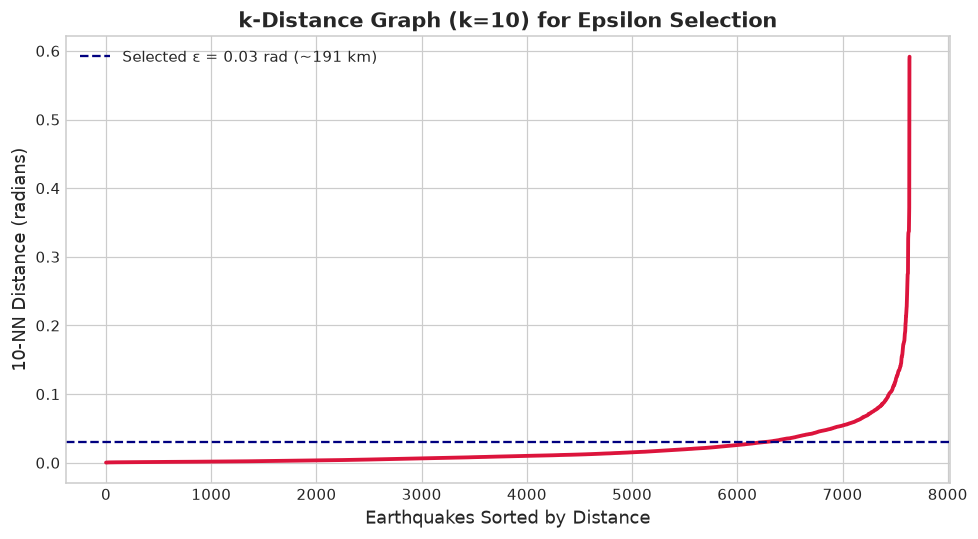
\includegraphics[width=0.72\textwidth]{figures/exp05_kdistance.png}
  \caption{The $k$-distance graph ($k = 10$); the knee at $\varepsilon = 0.03$ rad marks the
  transition from dense seismic zones to sparse isolated events.}
  \label{fig:exp05-kdist}
\end{figure}

\begin{figure}[htbp]
  \centering
  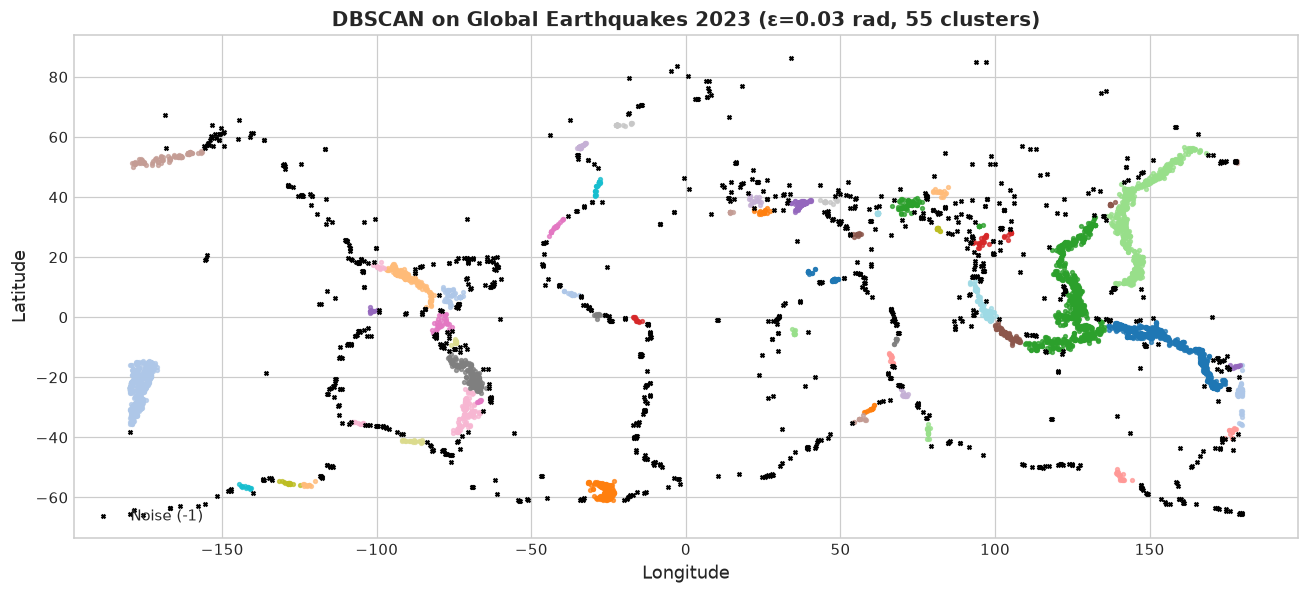
\includegraphics[width=0.95\textwidth]{figures/exp05_dbscan_map.png}
  \caption{DBSCAN clusters (colors) and noise (black crosses) on the global 2023 earthquake
  catalogue. The clusters trace the tectonically active plate boundaries.}
  \label{fig:exp05-map}
\end{figure}

With $\varepsilon = 0.03$ rad the algorithm finds 55 clusters and labels 13.5\% of the events
as noise. Smaller $\varepsilon$ fragments clusters and labels more events as noise; larger
$\varepsilon$ merges boundaries and reduces noise. The largest clusters correspond exactly to
known seismic zones, and the silhouette on non-noise events (3,000-event sample) is 0.326.

\section{Viva / Discussion Questions}
\begin{description}
  \item[Why does DBSCAN not require $K$?] Clusters are grown from density-connected core
  points, so their number and shape emerge from the data instead of being fixed in advance.
  \item[What does label $-1$ mean?] The point is neither a core nor a border point --- it lies
  in a sparse region and is treated as noise/outlier (here: isolated earthquakes).
  \item[Why can DBSCAN struggle with varying densities?] A single $\varepsilon$ that is small
  enough for a dense cluster fragments a sparse one, while one large enough for the sparse
  cluster merges the dense ones.
  \item[Why is haversine used instead of Euclidean distance?] Latitude/longitude are
  spherical coordinates; haversine gives true great-circle distances (radian inputs,
  $\varepsilon$ in radians).
  \item[How is $\varepsilon$ selected?] From the knee of the $k$-distance graph with
  $k = \texttt{min\_samples}$ (0.03 rad here).
\end{description}

\FloatBarrier
\section{Complete Code Listing}
% ===========================================================================
% exp05_dbscan.tex - complete code listings for Experiment 5
% Source: notebooks/02_density_based_learning.ipynb (executed)
% ===========================================================================

\begin{lstlisting}[style=mlcode,caption={Core numerical and plotting libraries}]
# ---- Core numerical and plotting libraries ----
import numpy as np
import pandas as pd
import matplotlib.pyplot as plt
import seaborn as sns

# ---- Density-based clustering algorithms ----
from sklearn.cluster import DBSCAN, HDBSCAN
# ---- Nearest-neighbor search (used to pick epsilon) ----
from sklearn.neighbors import NearestNeighbors
# ---- Evaluation metrics ----
from sklearn.metrics import silhouette_score

# Aesthetics setup (consistent look across all notebooks)
plt.style.use('seaborn-v0_8-whitegrid' if 'seaborn-v0_8-whitegrid' in plt.style.available else 'default')
plt.rcParams['font.sans-serif'] = 'DejaVu Sans'
plt.rcParams['figure.figsize'] = (11, 6)
plt.rcParams['figure.dpi'] = 110

np.random.seed(42)
print("Density-based libraries loaded successfully!")
\end{lstlisting}

\begin{lstlisting}[style=mlcode,caption={Load the real USGS earthquake catalogue (global, 2023)}]
# ---- Load the real USGS earthquake catalogue (global, 2023) ----
df = pd.read_csv('../data/earthquakes.csv')
print(f"Full catalogue (magnitude >= 4.0): {len(df):,} events")
print(df.head(3).to_string(index=False))

# Keep well-recorded moderate+ events: magnitude >= 4.5
quakes = df[df['mag'] >= 4.5].reset_index(drop=True)
print(f"\nAnalysed subset (magnitude >= 4.5): {len(quakes):,} events")

# ---- Convert epicenters to radians [latitude, longitude] ----
# scikit-learn's 'haversine' metric expects radian coordinates and computes
# great-circle distance on the sphere (correct for global data).
X_rad = np.radians(quakes[['latitude', 'longitude']].values)
print("Coordinate range (deg): lat", quakes.latitude.min(), "to", quakes.latitude.max(),
      "| lon", quakes.longitude.min(), "to", quakes.longitude.max())
\end{lstlisting}

\begin{lstlisting}[style=mlcode,caption={Choosing epsilon from the k-distance graph (haversine metric)}]
# ---- Choosing epsilon from the k-distance graph (haversine metric) ----
# Sorted distance to each event's k-th nearest neighbor. The knee marks the
# transition from dense seismic zones to sparse, isolated events.
min_samples = 10
nbrs = NearestNeighbors(n_neighbors=min_samples, metric='haversine').fit(X_rad)
distances, _ = nbrs.kneighbors(X_rad)
k_distances = np.sort(distances[:, -1])   # radians (0.03 rad = 191 km on Earth)

plt.figure(figsize=(9, 5))
plt.plot(k_distances, color='crimson', linewidth=2.5)
plt.title(f"k-Distance Graph (k={min_samples}) for Epsilon Selection", fontsize=14, fontweight='bold')
plt.xlabel("Earthquakes Sorted by Distance", fontsize=12)
plt.ylabel(f"{min_samples}-NN Distance (radians)", fontsize=12)
plt.axhline(y=0.03, color='navy', linestyle='--', label='Selected ε = 0.03 rad (~191 km)')
plt.legend()
plt.tight_layout()
plt.show()
\end{lstlisting}

\begin{lstlisting}[style=mlcode,caption={Fit DBSCAN with the chosen epsilon and MinPts}]
# ---- Fit DBSCAN with the chosen epsilon and MinPts ----
# DBSCAN grows clusters from core events, connects them via density-reachability,
# and labels everything else as noise (-1).
eps_selected = 0.03   # radians -> 0.03 * 6371 km ~ 191 km
dbscan = DBSCAN(eps=eps_selected, min_samples=min_samples, metric='haversine')
db_labels = dbscan.fit_predict(X_rad)

# Identify which events are core points (returned by the model) vs. border points
core_samples_mask = np.zeros_like(db_labels, dtype=bool)
core_samples_mask[dbscan.core_sample_indices_] = True

n_clusters_db = len(set(db_labels)) - (1 if -1 in db_labels else 0)
n_noise_db = np.sum(db_labels == -1)
print(f"DBSCAN: {n_clusters_db} clusters, {n_noise_db:,} noise events ({n_noise_db / len(X_rad) * 100:.1f}%)")

# ---- Visualize epicenters: clustered events in color, noise as black crosses ----
plt.figure(figsize=(12, 5.5))
palette = sns.color_palette("tab20", max(n_clusters_db, 1))
for k in range(n_clusters_db):
    mask = db_labels == k
    plt.scatter(quakes.longitude[mask], quakes.latitude[mask], s=6, color=palette[k % 20], alpha=0.75)

noise_mask = db_labels == -1
plt.scatter(quakes.longitude[noise_mask], quakes.latitude[noise_mask], s=6, color='black', marker='x', label='Noise (-1)')
plt.title(f"DBSCAN on Global Earthquakes 2023 (ε={eps_selected} rad, {n_clusters_db} clusters)", fontsize=13, fontweight='bold')
plt.xlabel("Longitude", fontsize=12)
plt.ylabel("Latitude", fontsize=12)
plt.legend(loc='lower left')
plt.tight_layout()
plt.show()
\end{lstlisting}

\begin{lstlisting}[style=mlcode,caption={Parameter sensitivity: DBSCAN under several (eps, min\_samples) settings}]
# ---- Parameter sensitivity: DBSCAN under several (eps, min_samples) settings ----
# The manual requires at least two settings so the effect of eps can be discussed.
print("eps (rad)   approx km   clusters   noise %")
for eps_test in [0.02, 0.03, 0.05]:
    lbl = DBSCAN(eps=eps_test, min_samples=10, metric='haversine').fit_predict(X_rad)
    n_clusters_test = len(set(lbl)) - (1 if -1 in lbl else 0)
    noise_pct = (lbl == -1).mean() * 100
    print(f"  {eps_test:.2f}       {eps_test * 6371:5.0f}      {n_clusters_test:3d}      {noise_pct:5.1f}%")
\end{lstlisting}


% ---------------------------------------------------------------------------
\chapter{HDBSCAN}\label{exp:06}

\runninghead{Experiment 6: HDBSCAN}

\quickfacts
  {Dataset}{USGS earthquakes 2023 (7,638 events, magnitude $\ge$ 4.5; radians + haversine)}
  {Key parameters}{\texttt{min\_cluster\_size} = 50, \texttt{min\_samples} = 10; no global $\varepsilon$}
  {Headline result}{40 clusters, 21.5\% noise; silhouette 0.631 on non-noise events}

\section{Objective}
Apply hierarchical density-based clustering to discover clusters of different densities and
identify noise without selecting a global radius.

\section{Suggested Dataset}
The same real earthquake catalogue as Experiment 5 (7,638 events, radians + haversine metric).

\section{Required Libraries}
scikit-learn, numpy, pandas, matplotlib.

\section{Brief Theory}
HDBSCAN removes the need for a global $\varepsilon$ by building a hierarchy over all density
levels:
\begin{enumerate}
  \item compute the \textbf{core distance} $d_{\text{core}}(p)$ --- the distance to a point's
        $k$-th nearest neighbor;
  \item define the \textbf{mutual reachability distance}
        $d_{\text{mreach}}(a,b) = \max\{d_{\text{core}}(a), d_{\text{core}}(b), d(a,b)\}$;
  \item build a \textbf{minimum spanning tree} over the mutual-reachability graph;
  \item convert the MST into a cluster hierarchy and condense it, tracking cluster births and
        deaths;
  \item keep the clusters with the highest \textbf{stability}
        $S(C) = \sum_{p \in C} (\lambda_p - \lambda_{\text{birth}}(C))$.
\end{enumerate}
The result is a flat clustering with per-point membership probabilities and noise labels, with
no radius to tune.

\section{Procedure}
\begin{enumerate}
  \item Reuse the prepared radian coordinates.
  \item Fit HDBSCAN with \texttt{min\_cluster\_size} = 50 and \texttt{min\_samples} = 10.
  \item Count clusters and noise events; inspect the membership probabilities.
  \item Visualize the partition.
  \item Compare with DBSCAN.
  \item Discuss the effect of \texttt{min\_cluster\_size}.
\end{enumerate}

\section{Reference Implementation}
\begin{codebox}[title={HDBSCAN on the earthquake data (no global epsilon)}]
hdb = HDBSCAN(min_cluster_size=50, min_samples=10, metric='haversine', copy=False)
hdb_labels = hdb.fit_predict(X_rad)
\end{codebox}

\section{Evaluation / Expected Output}
\begin{table}[htbp]
  \centering
  \caption{Density-based comparison on the 2023 earthquake catalogue.}
  \begin{tabular}{|l|r|r|r|r|}
    \hline
\rowcolor{mlblue!8}    \textbf{Algorithm} & \textbf{Clusters} & \textbf{Noise} & \textbf{Largest cluster} & \textbf{Silhouette} \\
    \hline
    DBSCAN ($\varepsilon = 0.03$) & 55 & 13.5\% & 1,629 & 0.326 \\
\hline
    HDBSCAN & 40 & 21.5\% & 560 & \best{0.631} \\
    \hline
  \end{tabular}
\end{table}

\begin{figure}[htbp]
  \centering
  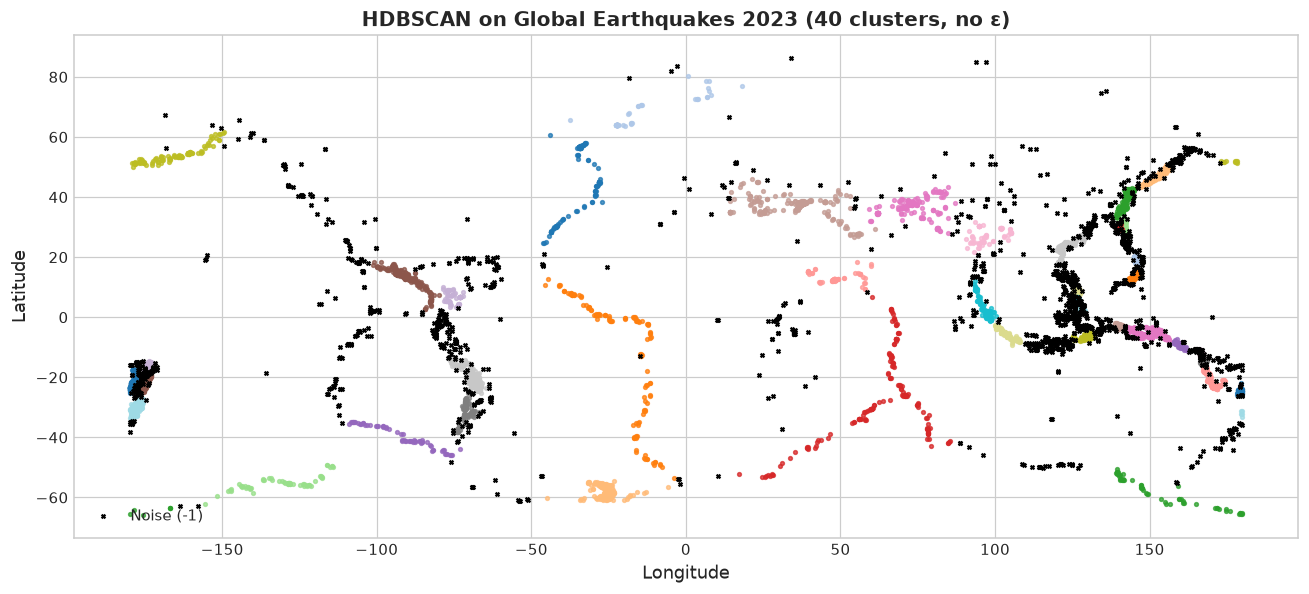
\includegraphics[width=0.95\textwidth]{figures/exp06_hdbscan_map.png}
  \caption{HDBSCAN clusters and noise on the same catalogue; adaptive density splits the
  long DBSCAN arc clusters into compact, well-separated groups.}
  \label{fig:exp06-map}
\end{figure}

HDBSCAN needs no $\varepsilon$ and handles the varying density along plate boundaries better
than DBSCAN; it is more conservative (21.5\% vs.\ 13.5\% noise) because a cluster must remain
stable across density scales. Its silhouette is roughly double DBSCAN's because the
fixed-$\varepsilon$ algorithm chains entire arc-shaped boundaries into single elongated
clusters. Membership probabilities are high ($>0.9$) deep inside seismic zones and lower near
cluster edges.

\section{Viva / Discussion Questions}
\begin{description}
  \item[What is hierarchical about HDBSCAN?] It constructs a full hierarchy of density-based
  clusters across all density levels and then condenses it by tracking cluster birth and death,
  keeping only the most stable clusters.
  \item[What does membership probability mean?] A per-point confidence that it belongs to its
  assigned cluster, derived from the point's persistence as the density threshold changes;
  low values indicate borderline points.
  \item[Why is HDBSCAN useful for variable-density data?] Clusters are selected by stability
  across density levels rather than by one global $\varepsilon$, so dense and sparse clusters
  can coexist.
  \item[What does \texttt{min\_cluster\_size} control?] The smallest group that may become a
  cluster; increasing it reduces the number of small clusters, decreasing it fragments the map.
\end{description}

\FloatBarrier
\section{Complete Code Listing}
% ===========================================================================
% exp06_hdbscan.tex - complete code listings for Experiment 6
% Source: notebooks/02_density_based_learning.ipynb (executed)
% ===========================================================================

\begin{lstlisting}[style=mlcode,caption={Core numerical and plotting libraries}]
# ---- Core numerical and plotting libraries ----
import numpy as np
import pandas as pd
import matplotlib.pyplot as plt
import seaborn as sns

# ---- Density-based clustering algorithms ----
from sklearn.cluster import DBSCAN, HDBSCAN
# ---- Nearest-neighbor search (used to pick epsilon) ----
from sklearn.neighbors import NearestNeighbors
# ---- Evaluation metrics ----
from sklearn.metrics import silhouette_score

# Aesthetics setup (consistent look across all notebooks)
plt.style.use('seaborn-v0_8-whitegrid' if 'seaborn-v0_8-whitegrid' in plt.style.available else 'default')
plt.rcParams['font.sans-serif'] = 'DejaVu Sans'
plt.rcParams['figure.figsize'] = (11, 6)
plt.rcParams['figure.dpi'] = 110

np.random.seed(42)
print("Density-based libraries loaded successfully!")
\end{lstlisting}

\begin{lstlisting}[style=mlcode,caption={Load the real USGS earthquake catalogue (global, 2023)}]
# ---- Load the real USGS earthquake catalogue (global, 2023) ----
df = pd.read_csv('../data/earthquakes.csv')
print(f"Full catalogue (magnitude >= 4.0): {len(df):,} events")
print(df.head(3).to_string(index=False))

# Keep well-recorded moderate+ events: magnitude >= 4.5
quakes = df[df['mag'] >= 4.5].reset_index(drop=True)
print(f"\nAnalysed subset (magnitude >= 4.5): {len(quakes):,} events")

# ---- Convert epicenters to radians [latitude, longitude] ----
# scikit-learn's 'haversine' metric expects radian coordinates and computes
# great-circle distance on the sphere (correct for global data).
X_rad = np.radians(quakes[['latitude', 'longitude']].values)
print("Coordinate range (deg): lat", quakes.latitude.min(), "to", quakes.latitude.max(),
      "| lon", quakes.longitude.min(), "to", quakes.longitude.max())
\end{lstlisting}

\begin{lstlisting}[style=mlcode,caption={Fit HDBSCAN (no global epsilon required)}]
# ---- Fit HDBSCAN (no global epsilon required) ----
# min_cluster_size = smallest group considered a cluster; min_samples controls conservativeness.
hdb = HDBSCAN(min_cluster_size=50, min_samples=10, metric='haversine', copy=False)
hdb_labels = hdb.fit_predict(X_rad)

n_clusters_hdb = len(set(hdb_labels)) - (1 if -1 in hdb_labels else 0)
n_noise_hdb = np.sum(hdb_labels == -1)
print(f"HDBSCAN: {n_clusters_hdb} clusters, {n_noise_hdb:,} noise events ({n_noise_hdb / len(X_rad) * 100:.1f}%)")

# ---- Visualize the HDBSCAN partition ----
plt.figure(figsize=(12, 5.5))
palette = sns.color_palette("tab20", max(n_clusters_hdb, 1))
for k in range(n_clusters_hdb):
    mask = hdb_labels == k
    plt.scatter(quakes.longitude[mask], quakes.latitude[mask], s=6, color=palette[k % 20], alpha=0.75)

noise_mask = hdb_labels == -1
plt.scatter(quakes.longitude[noise_mask], quakes.latitude[noise_mask], s=6, color='black', marker='x', label='Noise (-1)')
plt.title(f"HDBSCAN on Global Earthquakes 2023 ({n_clusters_hdb} clusters, no ε)", fontsize=13, fontweight='bold')
plt.xlabel("Longitude", fontsize=12)
plt.ylabel("Latitude", fontsize=12)
plt.legend(loc='lower left')
plt.tight_layout()
plt.show()
\end{lstlisting}

